%
% iteration.tex
%
% (c) 2020 Prof Dr Andreas Müller, Hochschule Rapperswil
%
\section{Iteration
\label{buch:section:iteration}}
\rhead{Iteration}
Die meisten numerischen Problemlösungen mit einem Computer nutzen deren
Fähigkeit aus, dieselbe Rechnung immer wieder zu wiederholen, bis zum
Beispiel die gewünschte Genauigkeit erziehlt ist.
\index{Iteration}%
Es lohnt sich daher ganz unabhängig irgendwelchen Einschränkungen 
der Computer-Hardware zu überlegen, was passiert, wenn man eine
Funktion $f\colon \mathbb R\to\mathbb R$ immer wieder auf ihren eigenen
Output anwendet, wie das zum Beispiel der Code in einer Schleife
bei jedem Durchlauf macht.
\index{Hardware}%

In diesem Abschnitt ist also
\[
f\colon \mathbb{R}\to\mathbb{R} : x\mapsto f(x)
\]
eine differenzierbare Funktion.
\index{Funktion!differenzierbar}%
\index{differenzierbare Funktion}%
Mit einem gegebenen Startwert $x_0\in\mathbb R$ lässt sich durch
wiederholte Anwendung von $f$ die Folge
\[
x_0,\; x_1 = f(x_0),\; x_2 = f(x_1),\; x_3 = f(x_2),\; x_4 = f(x_3),\dots
\]
konstruieren.
\index{Iterationsfolge}%

Ist der Punkt $x^*$ ein {\em Fixpunkt} der Funktion $f(x)$, ist also
$f(x^*)=x^*$,
\index{Fixpunkt}%
dann ist die mit $x_0=x^*$ gebildete Iterationsfolge konstant.
Es stellt sich damit automatisch die Frage, was mit einem von $x^*$
abweichenden Startwert passiert.
Entfernen sich die Werte $x_k$ von $x^*$
oder konvergiert die Folge am Ende gegen $x^*$?
\index{Konvergenz}%

%
% Beispiele
%
\subsection{Beispiele}
Wir illustrieren die verschiedenen Situation, die beim Iterieren der
Funktion $f$ auftreten können an einigen Beispielen.

\begin{beispiel}
\label{section:beispiel:sqrtiteration}
Wir betrachten die Funktion 
\[
f\colon \mathbb{R}\to\mathbb{R} : x\mapsto \sqrt{x+2}
\]
Die Iterationsfolge ausgehend vom Startwert $x_0=0$ ist in
Tabelle~\ref{buch:table:sqrtiteration} dargestellt.
\index{Startwert}%

\begin{table}
\centering
\renewcommand\arraystretch{1.15}
%
% sqrtiteration.tex -- generated by sqrtiteration.m
%
% (c) 2020 Prof Dr Andreas Müller Hochschule Rapperswil
%
\begin{tabular}{|>{$}r<{$}|>{$}r<{$}|>{$}r<{$}|>{$}r<{$}|}
\hline
   k & x_k                           & \delta_k = 2-x_k     & \delta_{k-1} / \delta_{k} \\
\hline
  0 &             0.0000000000000000 &   2.0000000000000000 &        \\
  2 &             1.4142135623730951 &   0.5857864376269049 & 3.4142 \\
  3 & \underline{1.8}477590650225735 &   0.1522409349774265 & 3.8478 \\
  4 & \underline{1.9}615705608064609 &   0.0384294391935391 & 3.9616 \\
  5 & \underline{1.99}03694533443939 &   0.0096305466556061 & 3.9904 \\
  6 & \underline{1.997}5909124103448 &   0.0024090875896552 & 3.9976 \\
  7 & \underline{1.999}3976373924085 &   0.0006023626075915 & 3.9994 \\
  8 & \underline{1.9998}494036782890 &   0.0001505963217110 & 3.9998 \\
  9 & \underline{1.9999}623505652022 &   0.0000376494347978 & 4.0000 \\
 10 & \underline{1.99999}05876191524 &   0.0000094123808476 & 4.0000 \\
 11 & \underline{1.999997}6469034038 &   0.0000023530965962 & 4.0000 \\
 12 & \underline{1.999999}4117257645 &   0.0000005882742355 & 4.0000 \\
 13 & \underline{1.9999998}529314358 &   0.0000001470685642 & 4.0000 \\
 14 & \underline{1.9999999}632328584 &   0.0000000367671416 & 4.0000 \\
 15 & \underline{1.99999999}08082147 &   0.0000000091917853 & 4.0000 \\
 16 & \underline{1.999999997}7020537 &   0.0000000022979463 & 4.0000 \\
 17 & \underline{1.999999999}4255133 &   0.0000000005744867 & 4.0000 \\
 18 & \underline{1.9999999998}563782 &   0.0000000001436218 & 4.0000 \\
 19 & \underline{1.9999999999}640945 &   0.0000000000359055 & 4.0000 \\
 20 & \underline{1.99999999999}10236 &   0.0000000000089764 & 4.0000 \\
 21 & \underline{1.999999999997}7558 &   0.0000000000022442 & 3.9998 \\
 22 & \underline{1.999999999999}4389 &   0.0000000000005611 & 3.9996 \\
 23 & \underline{1.9999999999998}597 &   0.0000000000001403 & 3.9984 \\
 24 & \underline{1.9999999999999}649 &   0.0000000000000351 & 4.0000 \\
 25 & \underline{1.99999999999999}11 &   0.0000000000000089 & 3.9500 \\
 26 & \underline{1.999999999999997}8 &   0.0000000000000022 & 4.0000 \\
 27 & \underline{1.999999999999999}3 &   0.0000000000000007 & 3.3333 \\
 28 & \underline{1.9999999999999998} &   0.0000000000000002 & 3.0000 \\
 29 & \underline{2.0000000000000000} &   0.0000000000000000 &        \\
 30 & \underline{2.0000000000000000} &   0.0000000000000000 &        \\
\hline
\end{tabular}

\caption{Iterationsfolge für die Funktion $f(x)=\sqrt{x+2}$ ausgehend
vom Startwert $x_0=0$.
\label{buch:table:sqrtiteration}}
\end{table}

Die Werte konvergieren offenbar gegen den Wert $2$, 
In der dritten Spalte steht die Abweichung $\delta_k$ des $k$-ten Folgengliedes
vom Grenzwert $2$.
Mit jeder Iteration wird der Fehler um den Faktor 4 kleiner, wie die
vierte Spalte zeigt, in der Quotient aufeinanderfolgender Fehler
berechnet ist.

Dieses Verhalten des Fehlers kann man auch analytisch verstehen.
Nehmen wir an, dass $x_n = 2 + \delta_n$ und versuchen wir 
$x_{n+1}$ zu berechnen.
Indem wir die Funktion $f(x)$ im Punkt $x=2$ mit Hilfe der Ableitung
linear approximieren, erhalten wir wegen
\[
f'(x) = \frac{1}{2\sqrt{x+2}}
\]
den Wert
\[
x_{n+1} = f(x_n) = f(2 + \delta_n)
\approx
f(2) + f'(2)\cdot \delta_n
2 + \underbrace{\frac14\cdot \delta_n}_{\displaystyle\approx\delta_{n+1}}
\]
für $x_{n+1}$.
Der Fehler von $x_{n+1}$ ist also $\delta_{n+1}\approx\frac14\delta_n$.
In jedem Iterationsschritt gewinnen wir daher etwa 2 bit Genauigkeit.
Für die 52 bit Mantisse des \texttt{double} Typs brauchen wir also
etwa 26 Iterationen.
\end{beispiel}

\begin{beispiel}
\label{buch:beispiel:logistisch3}
Wir betrachten die Funktion
\[
f(x) = 3x(1-x).
\]
\index{logistische Funktion!mit $\lambda=3$}%
Sie hat zwei Fixpunkte, die man durch Lösen der quadratischen
Gleichung
\index{quadratische!Gleichung}%
\[
f(x^*)=x^*
\quad\Rightarrow\quad
x^*=-3x^{*2}+3x^*
\quad\Rightarrow\quad
3x^{*2}-2x^*=3x^*(x^*-{\textstyle\frac23})=0
\quad\Rightarrow\quad
x^*=
\begin{cases}
0      &\\
\frac23&
\end{cases}
\]
findet.

Für einen Startwert $x_0$ nahe des Fixpunktes $x^*=0$ gilt
\[
f(\delta)
=
3\delta(1-\delta)
=
3\delta - 3\delta^2.
\]
Für kleine Werte von $\delta$ kann man den quadratischen Term vernachlässigen
und sieht, dass der Fehler durch die Iteration verdreifacht wird.
Konvergenz zu diesem Fixpunkt ist also nicht möglich.

Für den Fixpunkt $x^* = \frac23$ finden wir
\begin{equation}
f({\textstyle\frac23}+\delta)
=
3({\textstyle\frac23}+\delta)({\textstyle\frac13}-\delta)
=
\frac{(2+3\delta)(1-3\delta)}3
=
\frac{2-3\delta+9\delta^2}{3}
=
\frac23 - \delta  + 9\delta^2
\label{buch:equation:logistic3error}
\end{equation}
Der Fehler $\delta$ wird zu $ -\delta(1-9\delta) $, er ändert also sein
Vorzeichen.
\index{Fehler}%
Ist $\delta>0$ wird der Fehlerbetrag wird nur um den Faktor $1-9\delta < 1$
reduziert.
Ist aber $\delta <0$, dann ist $1-9\delta>0$, der Fehlerbetrag wird wieder
vergrössert.

Sei jetzt $\delta>0$, wir wollen den Fehler nach zwei Iterationsschritten
berechnen.
Nach dem ersten ist der Fehler $\delta(1-9\delta)$, nach dem zweiten
\[
\delta(1-9\delta)(1-\delta(1-9\delta))
=
\delta(1-18\delta + 162\delta^2-729\delta^3).
\]
Für kleines $\delta$ können die Terme höhrer als erster Ordnung
vernachlässigt werden und man kann schliessen, dass der Fehler nach
zwei Iterationen tatsächlich um den Faktor $(1-18\delta)$ kleiner
geworden ist.

\begin{figure}
\centering
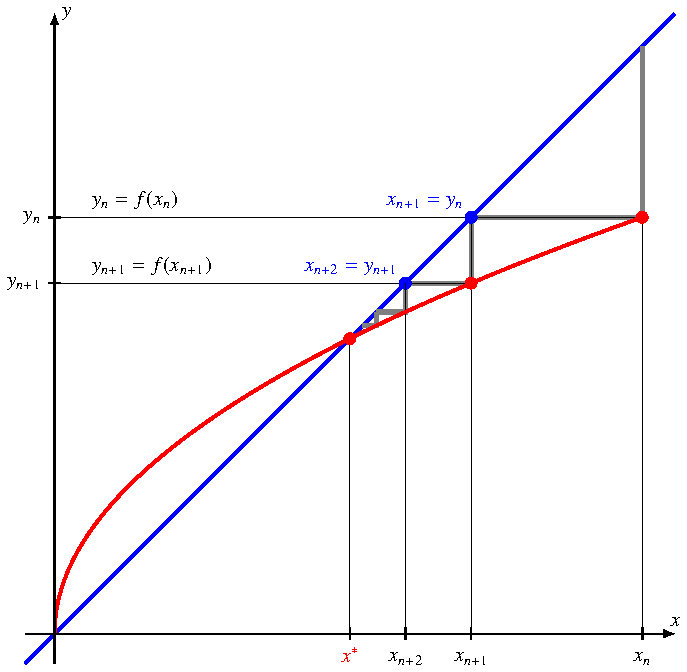
\includegraphics{chapters/10-arithmetik/figures/iteration.pdf}
\caption{Ein Fixpunkt $x^*$ der Funktion $f(x)$ manifestiert sich als
Schnittpunkt des Graphen $y=f(x)$ mit der $45^\circ$-Geraden.
\index{Schnittpunkt}%
\index{Graph}%
Die Iterationsfolge ausgehend von einem Startwert $x_0$ wird als
Treppenkurve zwischen dem Graphen von $f$ und der $45^\circ$-Geraden
sichtbar.
\index{Iterationsfolge}%
\label{buch:figure:iterationprinzip}}
\end{figure}

Wir möchten wissen, wieviele Iterationsschritte nötig sind, um eine
bestimmte Genauigkeit zu erreichen.
Wir möchten also den Fehler $\delta_{2n}$ vorgeben und das zugehörige
$n$ bestimmen.
Wie wir soeben berechnet haben, nimmt der Betrag des Fehlers zwischen
den Schritten $k$ und $k+2$ gemäss
\[
\delta_{k+2} = \delta_{k} (1-18\delta_k)
\]
um den Faktor $(1-18\delta_k)$ ab.
Es ist übersichtlicher, mit dem Logarithmus des Fehlers zu rechnen.
\index{Logarithmus}%
Dieser verändert sich gemäss
\[
\log \delta_{k+2}
=
\log \delta_{k} + \log(1-18\delta_k)
\approx
\log\delta_k - 18\delta_k,
\]
wobei wir für den zweiten Term die lineare Approximation aus der
Taylor-Reihe
\index{Taylor-Reihe}%
\index{lineare!Approximation}%
\index{Approximation!linear}%
\[
\log (1+x) = x - \frac{x^2}2 + \frac{x^3}3 -\dots
\]
von 
$\log x $ an der Stelle $x=1$ verwendet haben.
Zwischen $\delta_0$ und $\delta_{2n}$ bedeutet dies
\[
\log\delta_{2n}
=
\log\delta_0
-18
\sum_{k=0}^{n-1} \delta_{2k}
\qquad\Rightarrow\qquad
\frac1{18}
\log\frac{\delta_0}{\delta_{2n}}
=
\sum_{k=0}^{n-1}\delta_{2k}.
\]
Da der Fehler immer kleiner wir, kann man für eine erste grobe Abschätzung
\index{Abschätzung}%
der Summe auf der rechten Seite die grössten und kleinsten Terme
verwenden, um die Summe nach und unten und oben durch
\[
n\delta_{2n-2}
\le
\sum_{k=0}^{n-1}\delta_{2k}
\le
n\delta_0
\]
abzuschätzen.
Einsetzen ergibt
\[
n\delta_{2n-2}
\le
\frac{1}{18}
\log\frac{\delta_{0}}{\delta_{2n}}
\le
n\delta_0
\quad\Rightarrow\quad
\frac{1}{18\delta_0}
\log\frac{\delta_{0}}{\delta_{2n}}
\le
n
\le
\frac{1}{18\delta_{2n-2}}
\log\frac{\delta_{0}}{\delta_{2n}}
<
\frac{1}{18\delta_{2n}}
\log\frac{\delta_{0}}{\delta_{2n}}.
\]
Eine Verbesserung um zwei Stellen von $\delta_0=0.01$ auf $\delta_{2n}=0.0001$
braucht also zwischen $25$ und $2558$ Iterationen.
\end{beispiel}

%
% Graphische Analyse
%
\subsection{Graphische Analyse
\label{buch:section:graphischeanalyse}}
\index{graphische Analyse einer Iterationsfolge}%
\index{Iterationsfolge!graphische Konvergenzanalyse}%
Ein Fixpunkt der Funktion $f(x)$ manifestiert sich in einem 
Schnittpunkte des Graphen von $f$ mit der $45^\circ$-Geraden
$y=x$ wie in Abbildung~\ref{buch:figure:iterationprinzip}.
\index{Graph}%
\index{$45^\circ$-Gerade}%
\index{Schnittpunkt}%
Die Iterationsfolge $x_n$ kann graphisch wie folgt dargestellt
werden.
\index{Iterationsfolge}%
Ausgehend vom Wert $x_n$ auf der $x$-Achse folgt man der Vertikalen,
bis man auf den Graphen der Funktion $f$ trifft, dies liefert den
Wert $y_n=f(x_n)$.
Dieser soll jetzt als neuer $x$-Wert verwendet werden.
Dazu folgt man der Horizontalen bis zur $45^\circ$-Geraden,
die $x$-Koordinate des Schnittpunktes ist $x_{n+1}$.
So entsteht Treppenlinie in Abbildung~\ref{buch:figure:iterationprinzip}.
\index{Treppenlinie}%

%
% Konvergenzbedingung
%
\subsection{Konvergenzbedingung
\label{buch:iteration:subsection:konvergenzbedingung}}
%
% graphisch0.tex
%
% (c) 2020 Prof Dr Andreas Müller, Hochschule Rapperswil
%
\begin{figure}
\centering
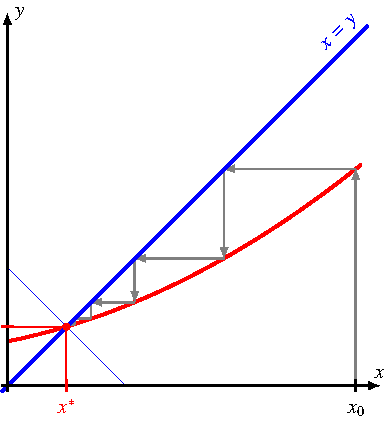
\includegraphics{chapters/10-arithmetik/figures/normal.pdf}
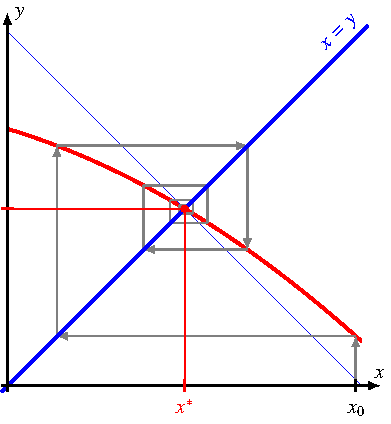
\includegraphics{chapters/10-arithmetik/figures/negativ.pdf}
\caption{Die Fixpunktiteration $x_{n+1}=f(x_n)$ konvergiert gegen
den Fixpunkt $x^*$ falls $|f'(x^*)|<1$ mit
mindestens linearer Konvergenzgeschwindigkeit.
\label{buch:figure:fixpunkt:normal}}
\end{figure}

%
% graphisch1.tex
%
% (c) 2020 Prof Dr Andreas Müller, Hochschule Rapperswil
%
\begin{figure}
\centering
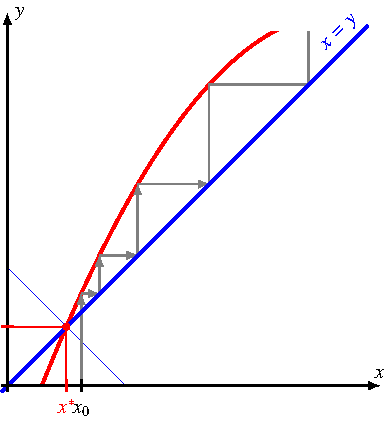
\includegraphics{chapters/10-arithmetik/figures/divergent.pdf}
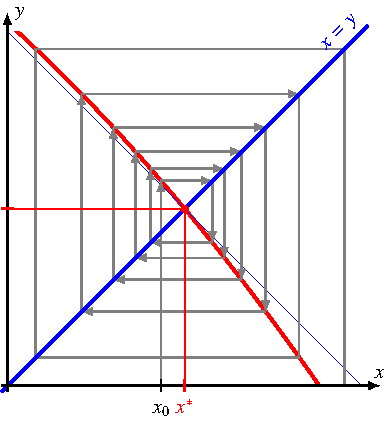
\includegraphics{chapters/10-arithmetik/figures/negdiv.pdf}
\caption{Die Fixpunktiteration $x_{n+1}=f(x_n)$ mit Fixpunkt $x^*$
divergiert für $|f'(x^*)|>1$.
\label{buch:figure:fixpunkt:divergent}}
\end{figure}

Aus der graphischen Analyse von Abschnitt~\ref{buch:section:graphischeanalyse}
kann man jetzt leicht Kriterien ableiten, wann die Iterationsfolge
konvergent ist.
Die Situation in Abbildung~\ref{buch:figure:iterationprinzip}
tritt zum Beispiel immer ein, wenn in einer Umgebung von $x^*$ 
der Graph der Funktion $f$ zwischen der horizontalen und der 
$45^\circ$-Geraden verläuft, oder anders ausgedrückt, wenn
\[
\begin{aligned}
x^* &< f(x) < x &&& &\text{für $x>x^*$ und} \\
x^* &> f(x) < x &&& &\text{für $x<x^*$}
\end{aligned}
\]
gilt.

Ist dagegen der Graph von $f$ in einer Umgebung von $x^*$ steiler als
die $45^\circ$-Gerade, dann gilt 
\begin{equation}
f(x) \;\begin{cases}
> x&\qquad\text{für $ x>x^*$}\\
< x&\qquad\text{für $ x<x^*$.}
\end{cases}
\label{buch:equation:konvergenzbedingung}
\end{equation}
Es folgt dann
\[
x_{n+1} = f(x_n)
\;
\begin{cases}
> x_n&\qquad \text{für $x_n>x^*$}\\
< x_n&\qquad \text{für $x_n<x^*$.}\\
\end{cases}
\]
In beiden Fällen ist $x_{n+1}$ weiter vom Fixpunkt $x^*$ entfernt
als $x_n$, die Folge kann also nicht konvergieren.
Die beiden Situationen sind in den Abbildungen
\ref{buch:figure:fixpunkt:normal} und
\ref{buch:figure:fixpunkt:divergent}
dargestellt.

Allerdings ist die Bedignung \ref{buch:equation:konvergenzbedingung}
noch etwas zu speziell.
Der Funktionswert $f(x_n)$ darf durchaus auch kleiner als $x^*$ werden,
wenn nur der Betrag der Differenz zu $x^*$ abnimmt, wenn also gilt
\begin{equation}
|x^* - f(x_n)| < |x^*-x_n|
\label{buch:equation:konvergenzbereich}
\end{equation}
Diese Bedingung ist genügend nahe bei $x^*$ erfüllt, wenn
$|f'(x^*)| < 1$ ist.
Andererseits liegt Divergenz vor, wenn 
\[
|x^* - f(x_n)| > |x^*-x_n|,
\]
was nahe bei $x^*$ erfüllt ist, wenn $|f'(x^*)|>1$ gilt.
Wir fassen diese Resultate im folgenden Satz zusammen.

\begin{satz}
\label{buch:satz:konvergenzkriterium}
\index{Konvergenzkriterium}%
\index{Iterationsfolge!Konvergenzkriterium}%
Die Iterationsfolge $x_{n+1}=f(x_n)$ der Funktion $f(x)$ mit Fixpunkt
$x^*=f(x^*)$ konvergiert für einen Startwert $x_0$ nahe genug bei $x^*$,
wenn $|f'(x^*)|<1$, sie divergiert, wenn $|f'(x^*)|>1$.
\end{satz}

%
% Die Logistische Gleichung
%
\subsection{Die logistische Gleichung
\label{buch:subsection:logistisch}}
Die logistische Gleichung ist 
\index{logistische Gleichung}%
\[
f_\lambda(x) = \lambda x(1-x)
\]
mit dem positiven Parameter $\lambda$.
Im Beispiel auf Seite~\pageref{buch:beispiel:logistisch3} haben wir
diese Funktion bereits einmal angetroffen mit dem Parameterwert
$\lambda=3$.
Eine detailliertere Untersuchung des Konvergenzverhaltes der Iterationen
dieser Funktionen ist im Kapitel~\ref{chapter:logistic} zu finden.

Der Graph von $f_\lambda(x)$ ist eine Parabel, die die $x$-Achse
in den Punkten $(0,0)$ und $(1,0)$ schneidet.
\index{Parabel}%
Das Maximum wird bei $x=\frac12$ angenommen und ist
$f_\lambda(\frac12)=\lambda/4$.
Die Funktion bildet also das Intervall $[0,1]$ wieder in das selbe Intervall
ab, wenn $0\le \lambda\le 4$.

Wir berechnen die Fixpunkte von $f_\lambda(x)$ im Intervall $[0,1]$, also
die Lösungen der quadratischen Gleichung
\[
x^*  = \lambda x^* (1-x^*)
\quad\Rightarrow\quad
\lambda x^{*2} +(1-\lambda)x^*
=
x^* (\lambda x^* + 1-\lambda) 
=0
\quad\Rightarrow\quad
x^*
=
\begin{cases}
0&\\
\displaystyle \frac{\lambda-1}{\lambda}.&
\end{cases}
\]
Für $\lambda<1$ gibt es keinen weitere Fixpunkt im Intervall $[0,1]$, für
$\lambda>1$ ist $(\lambda-1)/\lambda<1$ immer im Intervall.

Zur Beurteilung der Konvergenz der Iterationsfolge müssen wir die Ableitung
von $f_\lambda$ im Fixpunkt berechnen.
Die Ableitung ist $f'_\lambda(x)=\lambda (1-2x)$, also gilt in den Fixpunkten
\begin{align*}
f_\lambda'(0)
&=
\lambda
\\
f_\lambda\biggl(\frac{\lambda-1}{\lambda}\biggr)
&=
\lambda\biggl( 1-2
\biggl(\frac{\lambda-1}{\lambda}\biggr)\biggr)
=
\lambda-2(\lambda-1)
=
2-\lambda.
\end{align*}
Daraus liest man mit dem Konvergenzkriterium von
Satz~\ref{buch:satz:konvergenzkriterium} ab, dass Konvergenz zum Punkte
$(\lambda-1)/\lambda$ vorliegt für $\lambda \in (1,3)$.
\index{Konvergenzkriterium}%
Für $\lambda>3$ divergiert die Iterationsfolge.

Im Beispiel auf Seite~\pageref{buch:beispiel:logistisch3} haben wir
wir den Grenzfall $\lambda=3$ untersucht und festgestellt, dass die
Iterationsfolge gerade noch konvergiert, allerdings sehr langsam.
Man beachte, dass das Kriterium \eqref{buch:equation:konvergenzbereich}
in diesem Fall nicht erfüllt ist.
Für $\lambda<1$ konvergiert die Iterationsfolge zum Nullpunkt.

Wie verhält sich die Folge im Grenzfall $\lambda=1$?
Auch in diesem Grenzfall ist das Kriterium nicht erfüllt, wir müssen
das Problem als wieder gesondert analysieren.
Es gilt
\[
x_{n+1} = x_n(1-x_n) = x_n-x_n^2.
\]
Für $x_n>0$ folgt also, dass $0<x_{n+1} < x_n$ ist, die Folge wird also
konvergieren.
Allerdings ist die Konvergenz wieder ähnlich langsam wie im Falle
$\lambda=3$.
Für einen Wert $x_n<0$ ist allerdings $x_{n+1} = x_n - x_n^2 < x_n$,
d.~h.~die Folge divergiert.
Dieses Verhalten lässt sich auch allgemein formulieren.

\begin{satz}
\label{buch:satz:kritischekonvergenz}
Falls $f'(x^*)=1$, dann konvergiert die Iterationsfolge für einen
Startwert $x_0$ genügend nahe und grösser als $x^*$ wenn $f''(x^*)<0$ 
und sie divergiert für $f''(x^*)>0$.
Für einen Startwert genügend nahe und kleiner als $x^*$ dagegen
konvergiert die Iterationsfolge für $f''(x^*)<0$ und divergiert für
$f''(x^*)>0$.
\end{satz}

\begin{proof}[Beweis]
Wir entwickeln die Funktion $f$ im Punkt $x^*$ die Potenzreihe
\index{Potenzreihe}%
\begin{align*}
f(x^*+\delta)
&=
f(x^*) + f'(x^*)\cdot\delta + \frac12f''(x^*)\cdot \delta^* + O(\delta^3)
\\
&=
x^* + \delta + \frac12f''(x^*)\delta^2
\end{align*}
Die Entfernung zu Fixpunkt ist
\[
|f(x^*+\delta)-x^*|
\approx
|\delta  + \frac12f''(x^*)\delta^2|
=
|\delta|\cdot |1 + \frac12f''(x^*)\delta|.
\]
Ob die Entfernung wird genau dann grösser, wenn $f''(x^*)\delta$ positiv ist.
sie wird kleiner, wenn $f''(x^*)\delta$ negativ sind.
Der erste Fall tritt ein, wenn $\delta$ und $f''(x^*)$ gleiches
Vorzeichen haben.
Für Werte grösser als $x^*$ heisst das, dass $f''(x^*)>0$ sein muss.
Analog folgen alle anderen Fälle.
\end{proof}

Für den Fall $\lambda=3$ der logistischen Gleichung können wir den
folgenden Satz formulieren:

\begin{satz}
Falls $f'(x^*)=-1$, dann konvergiert die Iterationsfolge für einen
Startwert genügend nahe bei $x^*$, wenn $f''(x^*) <0$, sie divergiert,
wenn $f''(x^*)>0$.
\end{satz}

\begin{proof}[Beweis]
Wir verwenden wieder die Entwicklung
\begin{align*}
f(x_n)
&=
f(x^* +\delta_n)
=
f(x^*) + f'(x^*) \cdot \delta_n + \frac12 f''(x^*)\cdot \delta_n^2
+ \dots
=
x^* - \delta_n + \frac12f''(x^*)\delta_n^2 +\dots
\\
\delta_{n+1}
&=
-\delta + \frac12f''(x^*)\delta^2 \dots
\end{align*}
Daraus kann man zunächst ableiten, dass der Fehler bei jedem 
Iterationsschritt das Vorzeichen wechselt.
Wir berechnen den Fehler nach zwei solchen Schritten.
\begin{align*}
\delta_{n+2}
&=
-\delta_{n+1} + \frac12f''(x^*) \delta_{n+1}^2
=
\delta_n - \frac12f''(x^*) \delta_n^2
+
\frac12 f''(x^*) \bigl(-\delta_n + f''(x^*)\delta_n^2\bigr)^2
\\
&=
\delta_n 
-\frac12 f''(x^*)
\delta_n^2
+\frac12 f''(x^*)
\bigl( \delta_n^2 + 2f''(x^*)\delta_n^3 + f''(x^*)^2\delta_n^4\bigr)
\\
&=
\delta_n
+
f''(x^*)^2\delta_n^3
+
\frac12f''(x^*)^3\delta_n^4
+\dots
\\
&=
\delta_n (1 + f''(x^*)\delta_n^2)
\end{align*}
Die Terme höherer Ordnung als $3$ können für kleines $\delta_n$ 
vernachlässigt werden.
Nach zwei Iterationsschritten hat also der Fehler wieder das gleiche
Vorzeichen, aber der Betrag hat sich im den Faktor
\[
1+f''(x^*)\delta_n^2
\]
verändert.
Dieser Faktor ist genau dann $<1$, wenn $f''(x^*)<0$ ist.
\end{proof}

Ähnlich wie im Beispiel auf 
Seite~\pageref{buch:beispiel:logistisch3} kann man auch in diesem
Fall zeigen, dass die Konvergenz der Folge sehr langsam ist.

%
% Dritte Ableitung im Fixpunkt
%
\subsection{Dritte Ableitung im Fixpunkt
\label{buch:subsection:dritteableitungfixpunkt}}
\index{$f'''(x)$}%
\index{dritte Ableitung}%
\index{Ableitung!dritte}%
Die bisher zusammengetragenen Sätze decken die Fälle $|f'(x^*)|=1$ mit
nicht verschwindender zweiter Ableitung $f''(x^*)\ne 0$ ab.
In einigen Fällen ist Konvergenz nicht gesichert, doch wenn Konvergenz
vorliegt, dann ist sie sehr langsam.
Speziell an dieser Situation ist, dass
$f(x)-(x^* + f'(x^*)(x-x^*))$
das Vorzeichen in einer Umgebung von $x^*$ nicht wechselt.

Noch nicht untersucht wurde der Fall $f''(x^*)=0$.
Es ist klar, dass die Konvergenzgeschwindigkeit nicht schneller
werden kann.
\index{Konvergenzgeschwindigkeit}%
Für $f'''(x^*)\ne $ folgt zudem, dass in diesem Fall
$f(x)-(x^* + f'(x^*)(x-x^*))$
das Vorzeichen in einer Umgebung von $x^*$ wechselt.
Da aber das Iterationsverfahren sehr empfindlich darauf regiert, ob
der Graph von $f$ oberhalb oder unterhalb der Geraden $y=\pm x$ 
liegt, erwarten wir ein anderes Verhalten als im Fall $f''(x^*)\ne 0$.
%
% kubisch.tex
%
% (c) 2020 Prof Dr Andreas Müller, Hochschule Rapperswil
%
\begin{figure}
\centering
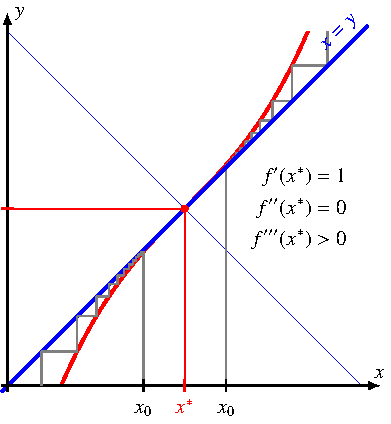
\includegraphics{chapters/10-arithmetik/figures/m1kp.pdf}
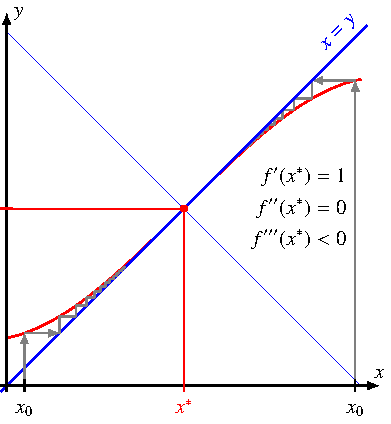
\includegraphics{chapters/10-arithmetik/figures/m1kn.pdf}
\caption{Die Fixpunktiteration $x_{n+1}=f(x_n)$ mit Fixpunkt $x^*$
mit $f'(x^*)=1$ und $f''(x^*)=0$ divergiert für $f'''(x^*)>0$
und konvergiert sehr langsam für $f'''(x^*)<0$.
\label{buch:figure:fixpunkt:abl1kub}}
\end{figure}
%
\begin{figure}
\centering
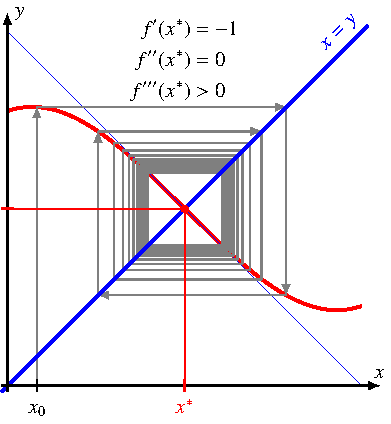
\includegraphics{chapters/10-arithmetik/figures/mnkp.pdf}
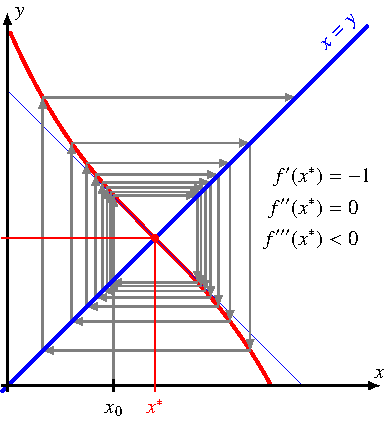
\includegraphics{chapters/10-arithmetik/figures/mnkn.pdf}
\caption{Die Fixpunktiteration $x_{n+1}=f(x_n)$ mit Fixpunkt $x^*$
mit $f'(x^*)=-1$ und $f''(x^*)=0$ konvergiert sehr langsam für $f'''(x^*)>0$
und divergiert für $f'''(x^*)<0$.
\label{buch:figure:fixpunkt:ablm1kub}}
\end{figure}
%
Alle möglichen Situationen sind in den
Abbildungen~\ref{buch:figure:fixpunkt:abl1kub} und
\ref{buch:figure:fixpunkt:ablm1kub} dargestellt.

Wir gehen also davon aus, dass sich $f$ in einer Umgebung von $x^*$
in der Form
\[
f(x^*+\delta)
\approx
\tilde{f}(x^*+\delta)
=
x^* + f'(x^*)\delta + \frac1{6}f'''(x^*) \delta^3
=
x^* + s\delta + a\delta^3
\]
entwickeln lässt, wobei $s=\pm 1$ und $a\ne 0$ ist.

Der Iterationsfehler $\delta_{n+1}$ verhält sich wie
\begin{align*}
x^* + \delta_{n+1}
&=
f(x_n)
=
f(x^* + \delta_n)
=
x^* + s\delta_n + a\delta_n^3 + O(\delta_n^4).
\\
\delta_{n+1}
&=
s\delta_n + a\delta_n^3 + O(\delta_n^4)
=
\delta_n(s+a\delta_n^2) + O(\delta_n^4)
=
s\delta_n\biggl(1+\frac{a}{s}\delta_n^2\biggr) + O(\delta_n^4)
\end{align*}
Da $\delta_n^2>0$ ist, ist der Klammerausdruck genügend nahe bei $x^*$
immer positiv.
Der Betrag des Fehlers verhält sich dann wie
\[
|\delta_{n+1}|
=
|\delta_n| \cdot \biggl(1 + \frac{a}{s}\delta_n^2\biggr) + O(\delta_n^4).
\]
Ob der Fehler bei der Iteration grösser oder kleiner wird, hängt also
einzig vom Vorzeichen von $a/s$ ab.
Ist $a/s > 0$, wird der Fehler grösser, die Iterationsfolge ist divergent,
ist $a/s < 0$, wird der Fehler kleiner, die Iterationsfolge konvergiert.
Wir fassen diese Resultate zusammen im folgenden Satz.

\begin{satz}
Falls $f\colon\mathbb R\to\mathbb R$ den Fixpunkt $x^*\in\mathbb R$ hat,
und $f'(x^*)=\pm1$, $f''(x^*)=0$ und $f'''(x^*)\ne 0$ ist, dann ist die
Iterationsfolge $x_{n+1}=f(x_n)$ konvergent, falls $f'(x^*)\cdot f'''(x^*)<0$
ist, gleichbedeutend damit, wenn $f'(x^*)$ und $f'''(x^*)$ verschiedene
Vorzeichen haben.
Wenn $f'(x^*)$ und $f'''(x^*)$ das gleiche Vorzeichen haben, dann ist
die Fixpunktiterationsfolge divergent.
\end{satz}

Abbildung~\ref{buch:figure:fixpunkt:abl1kub} zeigt die Situation $f'(x^*)=1$
während Abbildung~\ref{buch:figure:fixpunkt:ablm1kub} die Situation
$f'(x^*)=-1$ abdeckt.

